\documentclass[a4paper]{article}

%% Language and font encodings
\usepackage[english]{babel}
\usepackage[utf8x]{inputenc}
\usepackage[T1]{fontenc}
\usepackage{float}
\usepackage{tikz}
\usetikzlibrary{matrix}
\usepackage{algpseudocode} 

%% Sets page size and margins
\usepackage[a4paper,top=3cm,bottom=2cm,left=3cm,right=3cm,marginparwidth=1.75cm]{geometry}
\usepackage{amsmath}
\usepackage{amsthm}
\usepackage{amssymb}

\newtheorem{theorem}{Theorem}
\newtheorem{lemma}[theorem]{Lemma}

\begin{document}
\section*{1-D range query}
Describe how to efficiently perform one-dimensional range queries
for the data structures described in Problems 14 and 15. Given two keys $k_1 \leq k_2$, a
range query asks to report all the keys $k$ such that $k_1 \leq k \leq k_2$. Give an analysis of the
cost of the proposed algorithm, asking yourself whether it is output-sensitive, namely,
it takes $O(log_B N + R/B)$ block transfers where $R$ is the number of reported keys.
\\
\\
\textbf{SOLUTION}
\\
\\
The main idea in this exercise is to exploit the fact that keys at each level are stored sequentially, and they are sorted since we have a binary search tree\footnote{Notice that in both exercise we have provided a way to access the left and the right child}. Therefore, we can query the two keys $k_1,k_2$ using a simple binary search, and take all the keys that are in this range. Let's go in details for both data structures.
\begin{itemize}
\item[\textbf{Problem 14}] In this case the tree has been stored in an array, in which every layer of the tree is stored sequentially. For example for a binary tree we have: 
\begin{equation}
[root,L_1,R_1,L_{11},R_{11},L_{21},R_{22},...] \nonumber
\end{equation}
Therefore, the algorithm is going to search simultaneously the two keys $k_1,k_2$, and thus at each level is going through each layer. Here is going to find two position $t_1,t_2$ (in the case are not directly the keys) in which the algorithm is going to land, then all the keys we will find in the middle of $t_1,t_2$ are in the range $k_1,k_2$. 
\item[\textbf{Problem 15}] Here is a bit less intuitive but we exploit the same fact. Ones we have store implicitly the tree we are going to have a recursive layout of the tree, as shown in the picture below.
\begin{figure}[H]
\centering
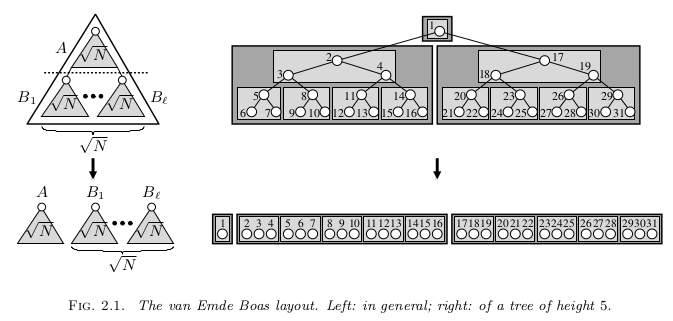
\includegraphics[scale=0.35]{VDB.png}
\end{figure}
Therefore at each splitting we are going to land (in the worst case) in two different blocks, and then we get all the keys that are between $k_1,k_2$ until we reach the keys in them self. At this point we get all the blocks that are in the middle. 
\end{itemize}
Notice that at certain point, in both cases we are going to end up with a sequence of key ($R$) stored sequentially. Therefore, we are going to have $2 log_B N$ access for two binary search and another $O(\frac{R}{B})$ to return the keys.
\end{document}